%%% template.tex
%%%
%%% This LaTeX source document can be used as the basis for your technical
%%% paper or abstract. Intentionally stripped of annotation, the parameters
%%% and commands should be adjusted for your particular paper - title, 
%%% author, article DOI, etc.
%%% The accompanying ``template.annotated.tex'' provides copious annotation
%%% for the commands and parameters found in the source document. (The code
%%% is identical in ``template.tex'' and ``template.annotated.tex.'')

\documentclass[conference]{acmsiggraph}

\TOGonlineid{45678}
\TOGvolume{0}
\TOGnumber{0}
\TOGarticleDOI{1111111.2222222}
\TOGprojectURL{}
\TOGvideoURL{}
\TOGdataURL{}
\TOGcodeURL{}

\title{Real-time shader-based rendering of grass}

\author {Kin Liu\\Manuel Reinfurt}
\pdfauthor{Kin Liu}

\keywords{radiosity, global illumination, constant time}

\begin{document}

%% \teaser{
%%   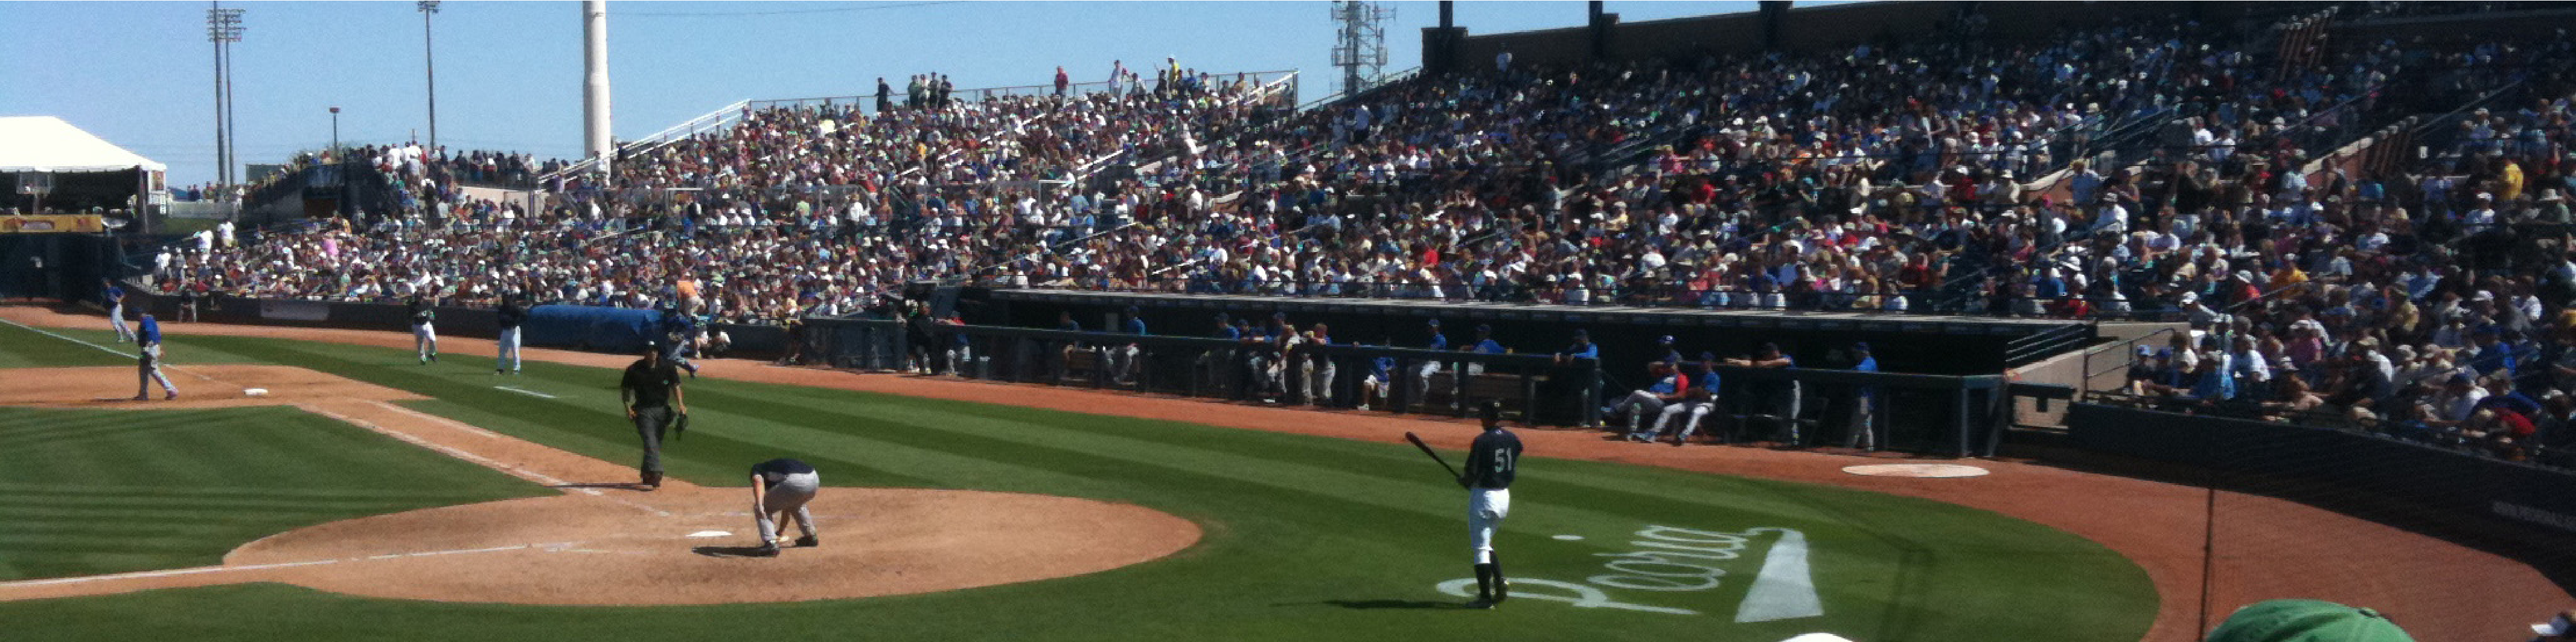
\includegraphics[height=1.5in]{images/sampleteaser}
%%   \caption{Spring Training 2009, Peoria, AZ.}
%% }

\maketitle

\begin{abstract}

The grass is the best.

\end{abstract}

\begin{CRcatlist}
  \CRcat{I.3.3}{Computer Graphics}{Three-Dimensional Graphics and Realism}{Display Algorithms}
  \CRcat{I.3.7}{Computer Graphics}{Three-Dimensional Graphics and Realism}{Radiosity};
\end{CRcatlist}

\keywordlist

%% Use this only if you're preparing a technical paper to be published in the 
%% ACM 'Transactions on Graphics' journal.

\TOGlinkslist

%% Required for all content. 

\copyrightspace

\section{Introduction}

Best

\begin{figure}[ht]
  \centering
  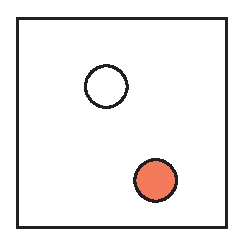
\includegraphics[width=1.5in]{images/samplefigure}
  \caption{Sample illustration.}
\end{figure}

\section{Methods}

Explain: General idea of grass, root points, density map. Terrain, height map, Y position displacement. Generating the grass blade with a dynamic number of vertices. Several grass patches in the grid instead of just one patch. Minimizing draw calls.

\begin{description}
  \item[CPU] \hfill \\
  The CPU will generate the root points out of the density map and create a single vertex buffer, that contains all roots. It will also slice the full grass grid into smaller patches, which can be controlled through constant buffers on the GPU.
  
  Since we also have static terrain, the root points will already contain the correct displaced Y position.
  \item[Vertex shader] \hfill \\
  The vertex shader is, in essence, a pass-through shader.
  \item[Geometry shader] \hfill \\
  All the hard work is done in the geometry shader. Since the geometry shader gets a single point as an input, it's job is to create a grass blade with a specified number of vertices. The geometry shader will also take care of calculating normals, level of detail, animation.
  \item[Pixel shader] \hfill \\
  To calculate the color, we use the basic Pong BDRF, combined with a texture and a randomized tint.
\end{description}

\section{Randomization}

The scene looks very artificial if the grass is laid out with exact distances, when each grass blade has the same tint, height or width. However, it is fairly difficult to generate random numbers on the GPU, which is why we have to use certain tricks to have fairly random grass properties. When laying out the root points, we can generate random positions using the CPU. Since these points are given to the geometry shader, and we kow that these positions are random, we can generate a random number between -1 and 1 using the following equation.

\begin{equation}
r = sin(\frac{\pi}2 * frac(root.x) + \frac{\pi}2 * frac(root.z))
\end{equation}

There is still a problem, though. Since we now only have one random number, the grass properties will be related to each other. If the grass is a bit higher, it will also be a bit browner.

INSERT non-randomized and randomized picture

\section{Animation}
Explain: Basic sine animation, Wind

\section{Wheat differences}
Explain: 

\section{Benchmarks}

FPS with different machines, root counts, level of detail settings and so on. Grapshs!

\section{Conclusion}

As you can see, shaders are... best.

\bibliographystyle{acmsiggraph}
\bibliography{template}
\end{document}
